\documentclass[10pt,draft]{article}
\usepackage[a4paper,left=2.54cm,top=2.54cm,right=2.54cm,bottom=2.54cm]{geometry}
\usepackage{fancyhdr}
\setlength{\headsep}{1.cm} % Adjust the space after the header
\usepackage{afterpage}
\usepackage{setspace}
\usepackage{bibspacing}
\usepackage{float}
\singlespacing

%%%% YOU CAN PUT YOUR OWN DEFINITIONS HERE
\newfont{\toto}{msbm10 at 12 pt}
\newfont{\ithd}{cmr9}
\newcommand{\equa}[1]{(\ref{eq:#1})}
\newcommand{\laeq}[1]{\label{eq:#1}}
\newcommand{\figu}[1]{\ref{fig:#1}} 
\newcommand{\lafi}[1]{\label{fig:#1}}
\newcommand{\fmo}{\tilde{U}}
\newcommand{\fve}{\tilde{u}}
\newcommand{\Dt}{\Delta t}

\newcommand{\R}{\mathbb{R}}
\newcommand{\Z}{\mathbb{Z}}
\newcommand{\si}[1]{\rm\scriptscriptstyle{#1}}
%%%% END OF YOUR DEFINITIONS 

\pagestyle{fancyplain}
\renewcommand{\headrulewidth}{0pt}

\usepackage{amsmath,amsthm,amsfonts,amssymb}
\usepackage{physics}
\usepackage[pdftex]{graphicx}
\usepackage[T1]{fontenc}

%%%% CONFERENCE HEADER. REPLACE xxxx WITH 4-DIGIT PAPER NUMBER ASSIGNED BY CONFERENCE COMMITTEE.

\rhead{\ithd{\bf ICCFD12-2024-xxxx\\  \   \\}}
\lhead{\ithd{\bf Twelfth International Conference on \\      
Computational Fluid Dynamics (ICCFD12), \\
Kobe, Japan, July 14-19, 2024
}}


\usepackage{titling}
\setlength{\droptitle}{0em}  
\pretitle{\vspace{-4em}\begin{center}\LARGE}
\posttitle{\end{center}\vspace{-1em}}
\preauthor{\begin{center}\large}
\postauthor{\end{center}\vspace{-6em}}


\title{
\bf A Novel Energy-based Artificial Viscosity for Suppressing Numerical Oscillations in Discontinuous Galerkin and Flux Reconstruction Schemes
}
\author{
Weicheng Pei$^{*}$ and Yu-Xin Ren$^{*}$\\
Corresponding author: weicheng.pei@icloud.com\\
$^{*}$ Department of Engineering Mechanics, Tsinghua University, Beijing 100084, China
}
\date{}

\usepackage[colorlinks=true]{hyperref}
\usepackage[]{physics}

\begin{document}

%%%% TITLE
\maketitle
\afterpage{\fancyhead{}}

%%%% ABSTRACT AND KEYWORDS
%\vskip0.5cm
\centerline{
}
\vskip0.5cm 

%%%% MAIN PART
\section{Introduction}
To construct high-order schemes on unstructured meshes, the discontinuous Galerkin (DG) method \cite{Cockburn_2001,Hesthaven_2008} and the flux reconstruction (FR) method \cite{Huynh_2007,Huynh_2014} are two of the most popular choices in the community of computational fluid dynamics (CFD).
%
Besides the inherent compactness, these schemes are much easier to implement $p$-refinement than their finite difference and finite volume counterparts.
%
However, like other high-order schemes, numerical oscillations would appear near discontinuities or large gradients in the solution given by a DG or FR scheme, if no shock fitting or shock capturing mechanism were incorporated into it.
%

%
Various shock capturing techniques, such as limiters \cite{Zhong_2013,Zhu_2013,Zhu_2020,Zhu_2023,Li_2020}, filters \cite{Dzanic_2022} and artificial viscosities \cite{Persson_2006,Klockner_2011,Discacciati_2020}, have been developed for DG and FR schemes in the past two decades.
%
However, most of these methods are based on orthogonal (modal) expansions, which are less efficient than pure Lagrange (nodal) expansions.
%
Some of them are even built upon extrapolations, i.e. evaluating an approximating polynomial outside the element it belongs to, which impairs the compactness of DG and FR schemes.
%

%
In this paper, a novel artificial viscosity based on an energy measure of oscillation and its damping rate on a DG or FR element is developed.
%
The oscillation energy, which measures the amplitude of numerical oscillations on a given element, is obtained by evaluating the $L_2$-norm of the difference between the numerical solutions on the element and its neighbors.
%
The damping rate of this energy on an element can be derived under the assumptions of linear flux--gradient relation and constant viscosity distribution.
%
The value of viscosity for suppressing numerical oscillations is obtained by taking the ratio of the oscillation energy with respect to the product of its damping rate and prescribed time step.
%
Such element-wise constant viscosity distribution could optionally be reconstructed to be $C_0$ continuous on element interfaces.

\section{Methodology}
\subsection{Element-wise Polynomial Approximations}
To solve the two-dimensional conservation law
$$
\partial_{t}\,u+\partial_{\vec{r}}\vdot\vec{f}=0,\quad\partial_{\vec{r}}\vdot\vec{f}=\partial_{x}\,f^{x}+\partial_{y}\,f^{y},
$$
using a DG or FR scheme, one may first introduce a map from the physical coordinates to the parametric coordinates on each element:
$$
\underbrace{(x,y)}_{\vec{r}}\mapsto\underbrace{(\xi,\eta)}_{\vec{\rho}}
\implies
\begin{bmatrix}\partial_{\xi}\,\phi\\
\partial_{\eta}\,\phi
\end{bmatrix}=\underbrace{\begin{bmatrix}\partial_{\xi}\,x & \partial_{\xi}\,y\\
\partial_{\eta}\,x & \partial_{\eta}\,y
\end{bmatrix}}_{\underline{J}}\begin{bmatrix}\partial_{x}\,\phi\\
\partial_{y}\,\phi
\end{bmatrix}=\begin{bmatrix}\partial_{\xi}\,\vec{r}\\
\partial_{\eta}\,\vec{r}
\end{bmatrix}\vdot\partial_{\vec{r}}\,\phi,
$$
in which $\underline{J}$ is the Jacobian matrix of the coordinate map.
%
The conservation law in physical coordinates is then (optionally) transformed into the form in parametric coordinates:
$$
\partial_{t}\,U+\partial_{\vec{\rho}}\vdot\vec{F}=0,\quad\partial_{\vec{\rho}}\vdot\vec{F}=\partial_{\xi}\,F^{\xi}+\partial_{\eta}\,F^{\eta},
$$
in which
$$
U=u\,\underbrace{\det(\underline{J})}_{J},\quad\begin{bmatrix}F^{\xi}\\
F^{\eta}
\end{bmatrix}=J\,\underbrace{\begin{bmatrix}\partial_{x}\,\xi & \partial_{y}\,\xi\\
\partial_{x}\,\eta & \partial_{y}\,\eta
\end{bmatrix}}_{\underline{J}^{-1}}\begin{bmatrix}f^{x}\\
f^{y}
\end{bmatrix}=J\begin{bmatrix}\partial_{\vec{r}}\,\xi\\
\partial_{\vec{r}}\,\eta
\end{bmatrix}\vdot\vec{f}.
$$

To obtain an element-wise polynomial approximation of the solution, an orthonormal (modal) expansion or a Lagrange interpolation has to be introduced for $u$ or $U\equiv Ju$ on the $j$th element:
$$
u(\vec{r},t)\approx u_{j}^{h}(\vec{r},t)=\begin{cases}
\sum_{n=1}^{N}\hat{u}_{j,n}(t)\,\phi_{j,n}(\vec{\rho}), & \text{Lagrange interpolation},\\
\sum_{m=1}^{M}\tilde{u}_{j,m}(t)\,\psi_{j,m}(\vec{r}), & \text{orthonormal expansion},
\end{cases}
$$
in which $\phi_{j,n}$ is the Lagrange basis associated with the $n$th node (a.k.a. solution point) on the $j$th element, which satisfies the Kronecker delta property
$$
\phi_{j,m}(\vec{\rho}_{j,n})=\delta_{mn},\quad\forall (m,n)\in\{1,\dots,N\}^2,
$$
while $\psi_{j,m}$ is the $m$th orthonormal basis on the $j$th element, which satisfies the innerproduct delta property
$$
\langle\psi_{j,m}\vert\psi_{j,n}\rangle=\delta_{mn},\quad\forall (m,n)\in\{1,\dots,M\}^2.
$$
%
The coefficient $\hat{u}_{j,n}$ is the nodal value of the approximate solution, i.e. $\hat{u}_{j,n}=u_j^h(\vec{r}(\vec{\rho}_n), t)$,
while the coefficient $\tilde{u}_{j,m}$ is the projection of the approximate solution on the $m$th basis, i.e. $\tilde{u}_{j,m}=\ip{u_j^h}{\psi_{j,m}}$

The number of terms $N$ or $M$ in the summations, i.e. the dimension of the polynomial space, depends on the degree of solution $P$ and the dimension of physical space $D$.
%
For tensor-product elements, e.g. quadrangles, hexahedra, the dimension of a Lagrange basis is equal to the product of the number of solution points in each dimension, which leads to
$$
N(P,D)=(P+1)^D,
$$
%
For building the orthonormal basis (in physical coordinates), one usually apply the Gram--Schmidt process to the basis formed by monomials whose degrees are less than or equal to $P$, which leads to
$$
M(P,D)=\binom{P+D}{D}.
$$
%
In general, the dimension of a nodal basis is much larger than that of the modal basis with the same $(P,D)$.

\subsection{ODE Systems from the DG and FR Methods}
An ordinary differential equation (ODE) system can then be derived from either the DG method or the FR method.

\subsection{Direct Viscous Fluxes on Element Interfaces}
Once an element-wise polynomial approximation is applied to the solution $u$, the flux $f(u,\grad u)$ is generally discontinuous on the interfaces of adjacent elements.
%
For the convection term in a conservation law, it is now a common practice to invoke an exact or an approximate Riemann solver \cite{Toro_2009}.
However, methods for getting the common diffusion flux are still actively been developed.

%
For solving problems involving diffusion terms, people in the field of DG usually introduce a new variable $\vec{q} \equiv \grad u$ and transform the second-order partial differential equation (PDE) into a first-order PDE system.
%
Schemes for getting the common value of $\vec{q}$ on element interfaces are then designed.
%
The famous Bassi--Rebay (BR) methods \cite{Bassi_1997,Bassi_2005} and the more general local DG (LDG) method \cite{Cockburn_1998b} all apply this \emph{indirect} procedure.
%
Recently, a method called direct DG (DDG) \cite{Liu_2009_DDG,Cheng_2016,Yang_2019} is becoming more and more popular, due to the fact that it gives the common value of $\grad u$ \emph{directly} without introducing the auxillary variable $\vec{q}$.
%
The common gradients are obtained by adding the penalty on jumps of value and second-order derivatives to the averaged gradient:
$$
\begin{bmatrix}\partial_{x}\,u\\
\partial_{y}\,u
\end{bmatrix}_{\partial E}=\beta_{0}\,\Delta^{-1}\begin{bmatrix}n_{x}\,u\\
n_{y}\,u
\end{bmatrix}_{\mathrm{R}-\mathrm{L}}+\begin{bmatrix}\partial_{x}\,u\\
\partial_{y}\,u
\end{bmatrix}_{(\mathrm{R}+\mathrm{L})/2}+\beta_{1}\,\Delta
\begin{bmatrix}
n_x\,\partial^2_{xx}\,u + n_y\,\partial^2_{xy}\,u\\
n_x\,\partial^2_{yx}\,u + n_y\,\partial^2_{yy}\,u
\end{bmatrix}_{\mathrm{R}-\mathrm{L}},
$$
in which $\Delta$ is the characteristic length of the element, and the $\beta$'s are the penalty weights.
%

%
It is straight forward to apply the DDG method to polynomials given by orthonormal expansions defined in physical coordinates (i.e. $\vec{r}\equiv(x,y)$).
%
However, it is more expensive and error-prone to be applied to solutions using Lagrange interpolation in parametric coordinates (i.e. $\vec{\rho}\equiv(\xi,\eta)$).
%
If, the interpolation is applied to $u$, the second-order derivatives are
$$
\begin{aligned}\begin{bmatrix}\partial_{xx}^{2}\,u & \partial_{xy}^{2}\,u\\
\partial_{yx}^{2}\,u & \partial_{yy}^{2}\,u
\end{bmatrix} & =\underbrace{\underline{J}^{-1}\begin{bmatrix}\partial_{\xi}\\
\partial_{\eta}
\end{bmatrix}}_{\begin{bmatrix}\partial_{x}\\
\partial_{y}
\end{bmatrix}}\underbrace{\left(\mathinner{\begin{bmatrix}\partial_{\xi}\,u & \partial_{\eta}\,u\end{bmatrix}}\underline{J}^{-T}\right)}_{\begin{bmatrix}\partial_{x}\,u & \partial_{y}\,u\end{bmatrix}}\\
 & =\underline{J}^{-1}\mathinner{\begin{bmatrix}\partial_{\xi}\mathinner{\begin{bmatrix}\partial_{\xi}\,u & \partial_{\eta}\,u\end{bmatrix}}\\
\partial_{\eta}\mathinner{\begin{bmatrix}\partial_{\xi}\,u & \partial_{\eta}\,u\end{bmatrix}}
\end{bmatrix}}\underline{J}^{-T}+\underline{J}^{-1}\begin{bmatrix}\mathinner{\begin{bmatrix}\partial_{\xi}\,u & \partial_{\eta}\,u\end{bmatrix}}\partial_{\xi}\,\underline{J}^{-T}\\
\mathinner{\begin{bmatrix}\partial_{\xi}\,u & \partial_{\eta}\,u\end{bmatrix}}\partial_{\eta}\,\underline{J}^{-T}
\end{bmatrix},
\end{aligned}
$$
in which the derivatives of the Jacobian matrix
$$
\pdv{\underline{J}^{-T}}{\xi}=\left(-\underline{J}^{-1}\,\pdv{\underline{J}}{\xi}\,\underline{J}^{-1}\right)^{T},\quad
\pdv{\underline{J}^{-T}}{\eta}=\left(-\underline{J}^{-1}\,\pdv{\underline{J}}{\eta}\,\underline{J}^{-1}\right)^{T},
$$
should be precomputed and cached on each flux point.
%
%
If the interpolation is applied to $U\equiv Ju$, the second-order derivatives are more complex:
$$
\begin{aligned}\begin{bmatrix}\partial^2_{xx}\,u & \partial^2_{xy}\,u\\
\partial^2_{yx}\,u & \partial^2_{yy}\,u
\end{bmatrix} & =\underbrace{\underline{J}^{-1}\begin{bmatrix}\partial_{\xi}\\
\partial_{\eta}
\end{bmatrix}}_{\begin{bmatrix}\partial_{x}\\
\partial_{y}
\end{bmatrix}}\underbrace{\left(\mathinner{\begin{bmatrix}\partial_{\xi}\,U & \partial_{\eta}\,U\end{bmatrix}}\underline{J}^{-T}\,J^{-1}-\mathinner{\begin{bmatrix}\partial_{\xi}\,J & \partial_{\eta}\,J\end{bmatrix}}\underline{J}^{-T}\,J^{-2}\,U\right)}_{\begin{bmatrix}\partial_{x}\,u & \partial_{y}\,u\end{bmatrix}}\\
 & =\underline{J}^{-1}\mathinner{\begin{bmatrix}\partial_{\xi}\,\partial_{\xi}\,U & \partial_{\xi}\,\partial_{\eta}\,U\\
\partial_{\eta}\,\partial_{\xi}\,U & \partial_{\eta}\,\partial_{\eta}\,U
\end{bmatrix}}\underline{J}^{-T}\,J^{-1}+\cdots,
\end{aligned}
$$
%
$$
\begin{aligned}\partial_{\xi}\left(\mathinner{\begin{bmatrix}\partial_{\xi}\,U & \partial_{\eta}\,U\end{bmatrix}}\underline{J}^{-T}\,J^{-1}\right) & =\mathinner{\begin{bmatrix}\partial_{\xi}\,\partial_{\xi}\,U & \partial_{\xi}\,\partial_{\eta}\,U\end{bmatrix}}\underline{J}^{-T}\,J^{-1}\\
 & +\mathinner{\begin{bmatrix}\partial_{\xi}\,U & \partial_{\eta}\,U\end{bmatrix}}\left(\pdv{\underline{J}^{-T}}{\xi}\,J^{-1}+\underline{J}^{-T}\left(\partial_{\xi}\,J^{-1}\right)\right),
\end{aligned}
$$
$$
\begin{aligned}\partial_{\xi}\left(\mathinner{\begin{bmatrix}\partial_{\xi}\,J & \partial_{\eta}\,J\end{bmatrix}}\underline{J}^{-T}\,J^{-2}\,U\right) & =\mathinner{\begin{bmatrix}\partial_{\xi}\,\partial_{\xi}\,J & \partial_{\xi}\,\partial_{\eta}\,J\end{bmatrix}}\underline{J}^{-T}\,J^{-2}\,U\\
 & +\mathinner{\begin{bmatrix}\partial_{\xi}\,J & \partial_{\eta}\,J\end{bmatrix}}\left(\pdv{\underline{J}^{-T}}{\xi}\,J^{-2}\,U+\underline{J}^{-T}\,\pdv{J^{-2}}{\xi}\,U+\underline{J}^{-T}\,J^{-2}\,\pdv{U}{\xi}\right),
\end{aligned}
$$
in which, the derivatives of Jacobian determinant
$$
\pdv{J^{-1}}{\xi}=-J^{-2}\,\pdv{J}{\xi},\quad\pdv{J^{-2}}{\xi}=-2J^{-3}\,\pdv{J}{\xi},
$$
$$
\pdv{J}{\xi}=\pdv{\det(\underline{J})}{\xi}=\det(\underline{J})\tr(\underline{J}^{-1}\,\pdv{\underline{J}}{\xi})=J\tr(\underline{J}^{-1}\,\pdv{\underline{J}}{\xi}),
$$
should also be cached.

\subsection{Oscillation Energy}
To measure the numerical oscillations quantitatively, we define the oscillation energy on the $j$th element to be
$$
\Delta K_j = \int_{x_{j-1/2}}^{x_{j}}\left(u_{j}^{h}-u_{j-1}^{h}\right)^{2}\dd{x}+\int_{x_{j}}^{x_{j+1/2}}\left(u_{j}^{h}-u_{j+1}^{h}\right)^{2}\dd{x},
$$
which is the square of the $L_2$-norm of difference between the solution on $E_j$ and those on its immediate neighbors.
The integrals are as cheap as weighted summations of nodal values if solution points are also Gaussian quadrature points, which is a common practice in the DG spectral element method (SEM) \cite{Li_2020}.

\subsection{Artificial Viscosity}
To dissipate the oscillation energy just defined, we introduce an artificial viscosity term, which is linear to the gradient of solution, to the conservation law, which becomes
$$
\pdv{u}{t}+\pdv{f(u)}{x}=\pdv{x}\qty(\nu\pdv{u}{x}),\quad \nu \ge 0.
$$
The ODE system given by the DG or FR scheme becomes
$$
\dv{t}\ket{\hat{u}_{j}}=\cdots+\nu_{j}\left(\underline{D}_{j}\ket{\hat{u}_{j}}+\underline{E}_{j}\ket{\hat{u}_{j-1}}+\underline{F}_{j}\ket{\hat{u}_{j+1}}\right),
$$
where $\ket{\hat{u}_{j}}, \ket{\hat{u}_{j-1}}, \ket{\hat{u}_{j+1}}$ are column matrices formed by nodal values on $E_{j}, E_{j-1}, E_{j+1}$ respectively, and $ \underline{D}_{j}, \underline{E}_{j}, \underline{F}_{j} $ are constant square matrices given the spatial discretization and the numerical flux on element interfaces.
The dissipation rate of the kinetic energy is
$$
\dv{t}\underbrace{\frac{1}{2}\Vert u_{j}^{h}\Vert_{L_{2}(E_{j})}^{2}}_{K_{j}}=\bra{\hat{u}_{j}}\underline{W}_{j}\dv{t}\ket{\hat{u}_{j}}=\cdots+\nu_{j}\,\underbrace{\left(\bra{\hat{u}_{j}}\underline{W}_{j}\,\underline{D}_{j}\ket{\hat{u}_{j}}+\cdots\right)}_{G_{j}},
$$
where $\underline{W}_{j}$ is the diagonal matrix form by Gaussian quadrature weights.
The value of viscosity is
$$
\nu_{j}=\frac{\Delta K_{j}}{-G_{j}\,\tau}\impliedby\dv{t}K_{j}=\cdots+\nu_{j}\,G_{j},
$$
which means the oscillation energy $\Delta K_{j}$ is dissipated by the viscosity within a prescribed time range $\tau$.

\section{Results}
In this section, the effectiveness of the artificial viscosity proposed in the previous section is demonstrated by some standard test cases.
The computational domain is divided into $100$ elements uniformly.
A fifth-order ($p=4$) FR scheme using the $g_2$ correction function, which is equivalent to a DG SEM scheme of the same order of accuracy, is used for spatial discretization.
The resulting ODE system is solved by an explicit three-stage third-order strong stability preserving Runge--Kutta method.

\subsection{Shock Tube Problems}
Riemann problems, as well as their exact and approximate solvers, play a pivot role in the development of CFD schemes \cite{Toro_2009}.
Among the infinite number of Riemann problems of the 1D Euler system, the Sod problem with the initial condition
\begin{equation}
\mqty[\rho & u & p]_{t=0}
=
\begin{cases}
\mqty[1 & 0 & 1], &x<0,\\
\mqty[0.125 & 0 & 0.1], &x>0,\\
\end{cases}
\end{equation}
and the Lax problem in with the initial condition
\begin{equation}
\mqty[\rho & u & p]_{t=0}
=
\begin{cases}
\mqty[0.445 & 0.698 & 3.528], &x<0,\\
\mqty[0.5 & 0 & 0.571], &x>0,\\
\end{cases}
\end{equation}
are two of the most famous ones that are frequently used for testing shock capturing mechanisms.

Figure \ref{fig:sod} and \ref{fig:lax} gives the solution (the "Actual" curves) of these two problems at the moment ($t=0.5$ for Sod, $t=0.3$ for Lax) and the viscosity distributions for each characteristic variables at all time steps.
The "Expect" curves in these figures are the exact solutions obtained from analytical procedures.
\begin{figure}[H]
  \centering
  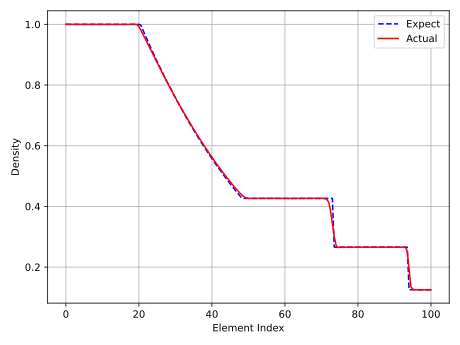
\includegraphics[width=.49\textwidth]{./sod/Frame100.pdf}
  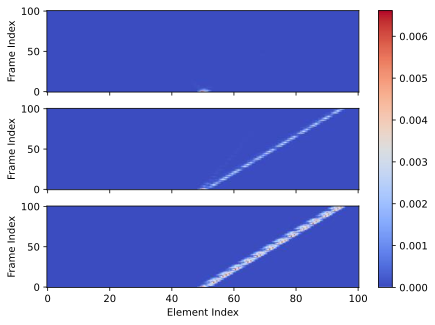
\includegraphics[width=.49\textwidth]{./sod/Viscosity.pdf}
  \caption{Solution and viscosity distribution of the Sod problem.}
  \label{fig:sod}
\end{figure}

\begin{figure}[H]
  \centering
  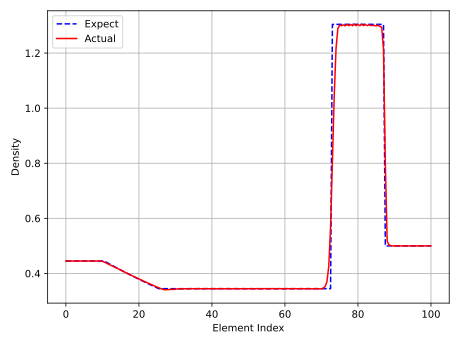
\includegraphics[width=.49\textwidth]{./lax/Frame100.pdf}
  \includegraphics[width=.49\textwidth]{./lax/Viscosity.pdf}
  \caption{Solution and viscosity distribution of the Lax problem.}
  \label{fig:lax}
\end{figure}

\subsection{The Shu--Osher Problem}\label{sec:shu_osher}

The Shu--Osher problem is designed to mimic the interaction of a running shock with a standing isentropic wave \cite{Shu_1989}.

The computational domain is $x\in[0, 10]$ with two no-reflection conditions applied at the left and right boundaries.
The time range of interest is $t\in[0, 1.8]$ with the initial condition set to be
\begin{equation}
\mqty[\rho & u & p]_{t=0}
=
\begin{cases}
\mqty[3.857143 & 2.629369 & 10.33333], &x\in[0,1);\\
\mqty[1+0.2\sin(5x) & 0 & 1], &x\in(1,10].
\end{cases}
\end{equation}

Figure \ref{fig:shu_osher} gives the solution (the \emph{Actual} curve) of this problem at the final ($t=1.8$) moment and the viscosity distribution for each characteristic variables at all time steps.
The \emph{Expect} curve in this figure is the approximate solution given by the same FR scheme with a $p$-weighted limiter \cite{Li_2020} on a finer mesh (200 elements).
\begin{figure}[H]
  \centering
  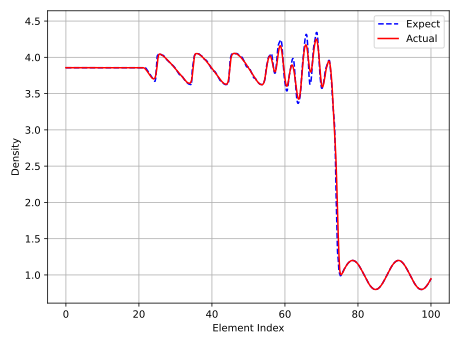
\includegraphics[width=.49\textwidth]{./shu_osher/final/Frame100.pdf}
  \includegraphics[width=.49\textwidth]{./shu_osher/final/Viscosity.pdf}
  \caption{Solution and viscosity distribution of the Shu--Osher problem.}
  \label{fig:shu_osher}
\end{figure}

These standard cases for testing shock capturing schemes show that the proposed mechanism is sufficiently large for suppressing numerical oscillations near physical discontinuities, such as shocks and contacts, while keeps negligible in other regions for maintaining the high-order accuracy of the DG or FR solution.

%%%% BIBLIOGRAPHY
\bibspacing=\dimen 100
\bibliographystyle{unsrt}
\bibliography{biblio}

\end{document}
